\subsection{UML diagrams}

\subsubsection{Context diagram}
The context diagram gives an overview over the applikation as a system. Here it is seen that there are four external entities: wristband, user, firebase and relatives. 
The first dataflow 'detect fall' goes from 'wristband' to the application. Then from the user 

\begin{figure}[H]
    \centering
    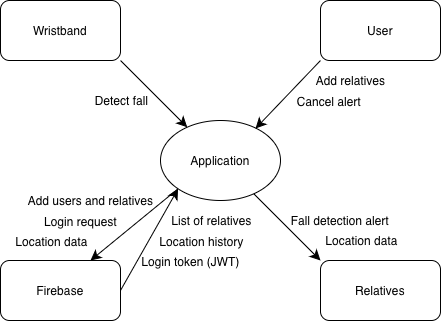
\includegraphics[width=0.75\linewidth]{report//images/Context.drawio.png}
    \caption{Context diagram over the application}
    \label{fig:placeholder}
\end{figure}

\subsubsection{User stories}

\begin{enumerate}
    \item As a user, I want to press the emergency button so that I can alert my relatives. 
    \item As a user, I want to send an alert when I fall so that I can notify my relatives. 
    \item As a user, I want to be able to cancel an alarm so that I don't have an active alarm when I am not in an emergency.
    \item As a user, I want to add multiple relatives to my notification list so that multiple relatives receive an alarm and help me. 
    \item As a user, I want to see the battery percentage in my app so that I can ensure my wristband is charged. 
\end{enumerate}
 

\subsubsection{Use case diagram}



\subsubsection{Data flow diagram}
\begin{figure} [H]
    \centering
    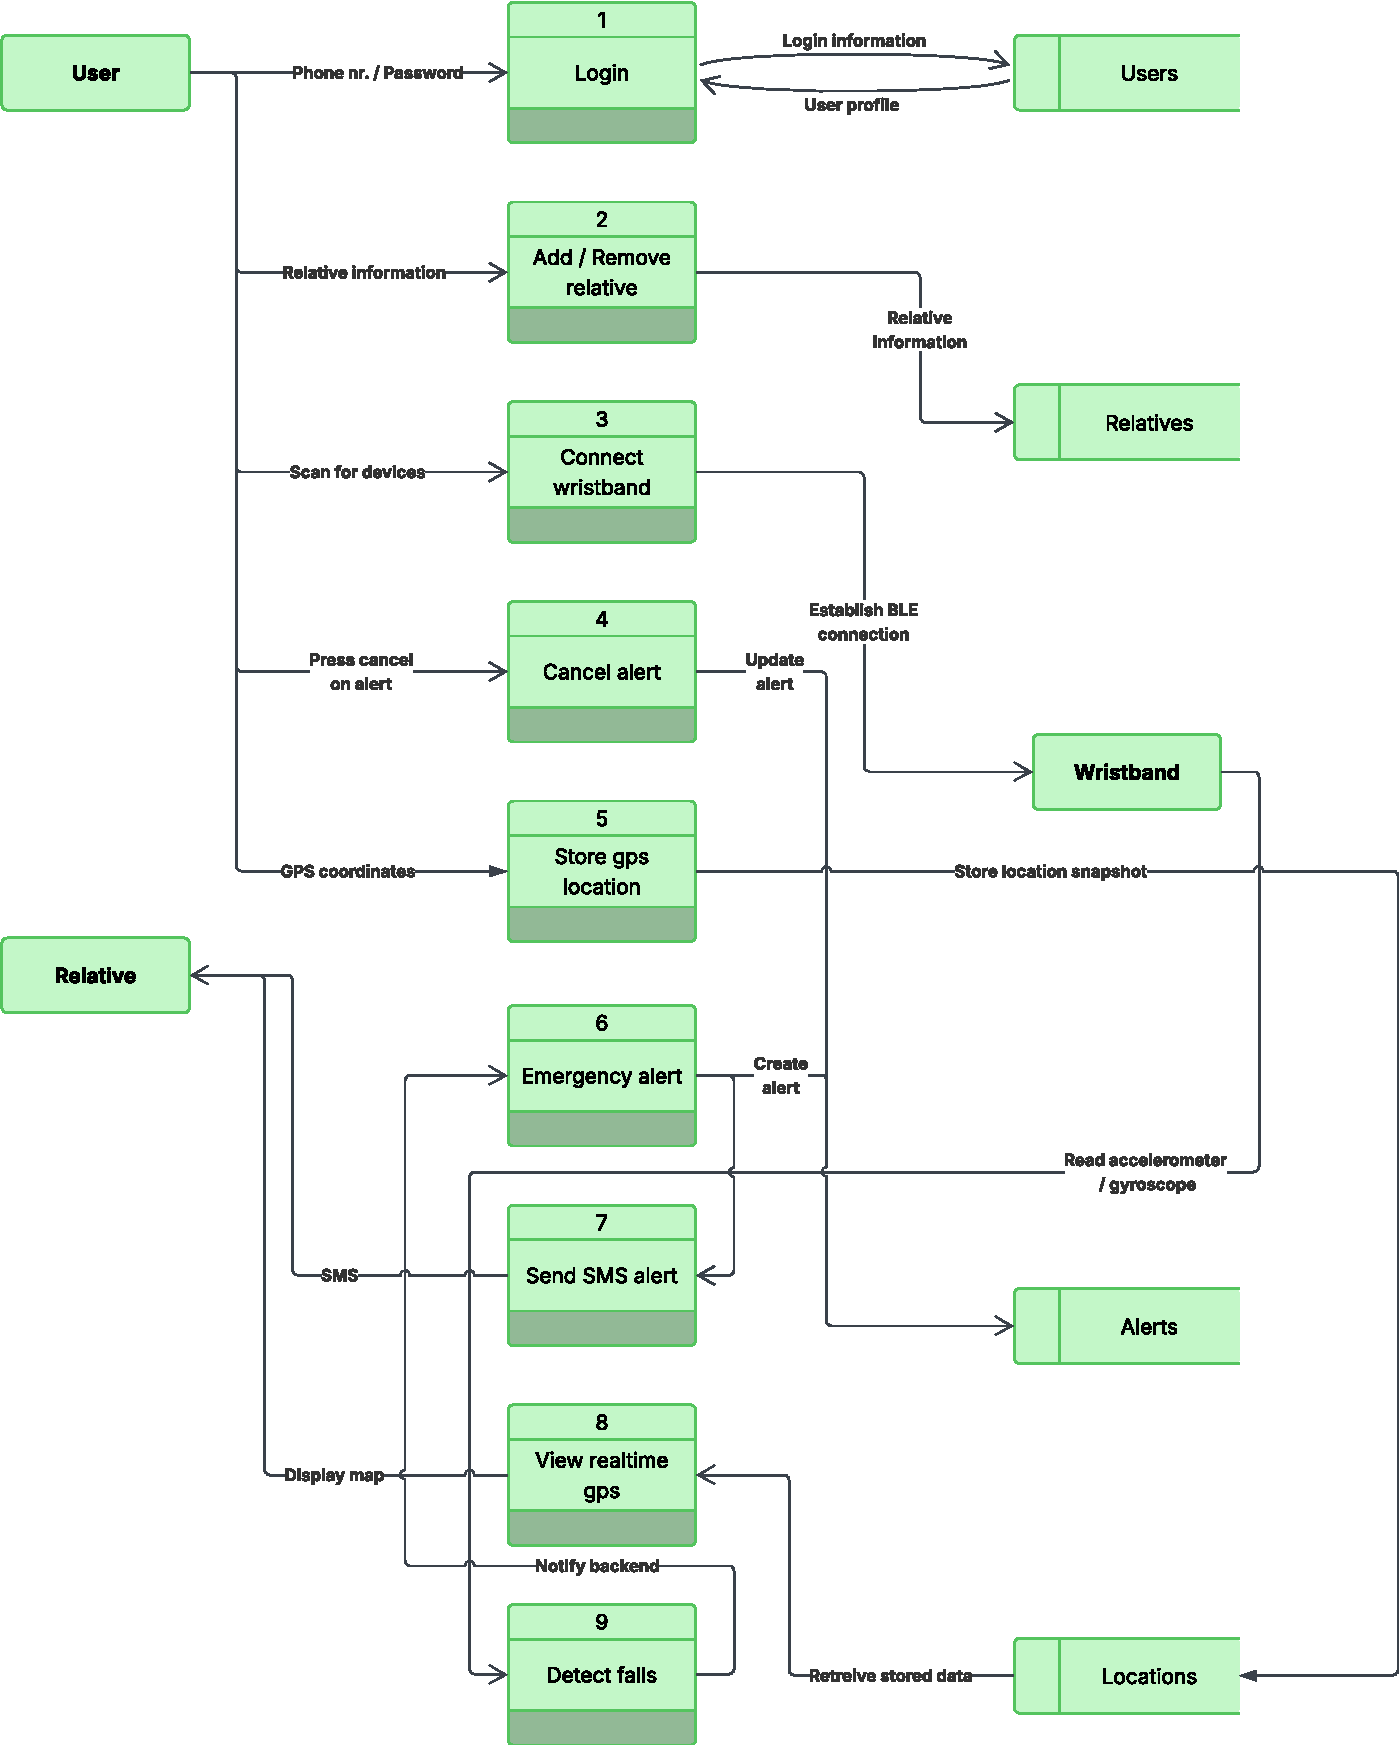
\includegraphics[width=1\linewidth]{Dataflow-Diagram-med-line-jumps.pdf}
    \caption{Enter Caption}
    \label{fig:placeholder}
\end{figure}

\subsubsection{Sequence diagram}
The sequence diagram below describes the sequence when a fall is detected. The fall is detected by the wristband, which then notifies the mobile app. The mobile app creates the alert, and a new entry is created in the database in the backend. After this, the backend alerts the relative, where they can then respond to the alert. The ‘optional’ shows how a fall can be cancelled by the user, in which case the mobile app cancels the alert, and the backend updates the corresponding database entry. After this, the backend notifies the relative, who can then contact the user regarding the cancelled alert.  
\begin{figure}[H]
    \centering
    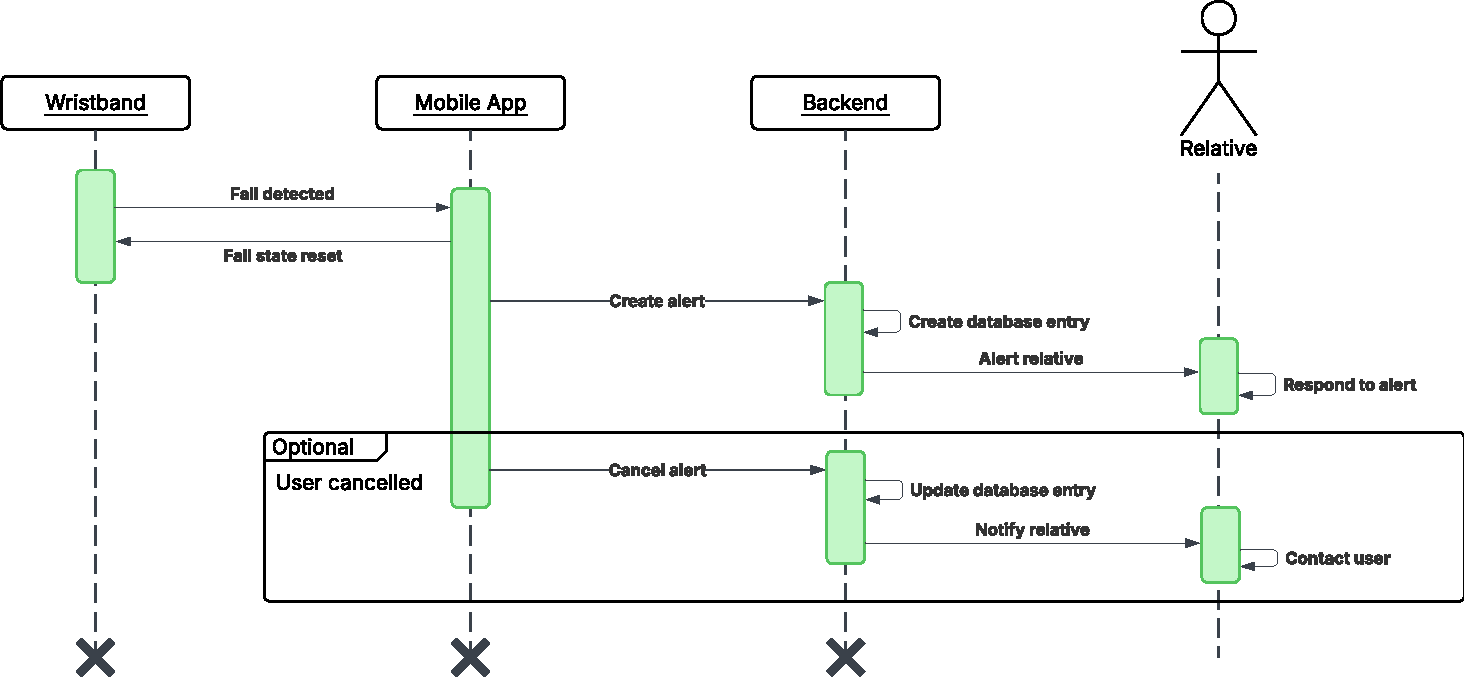
\includegraphics[width=1\linewidth]{Sequence-Diagram-Sequence-Diagram.pdf}
    \caption{Enter Caption}
    \label{fig:placeholder}
\end{figure}

\subsubsection{Deployment diagram}
In the following deployment diagram, 
\begin{figure} [H]
    \centering
    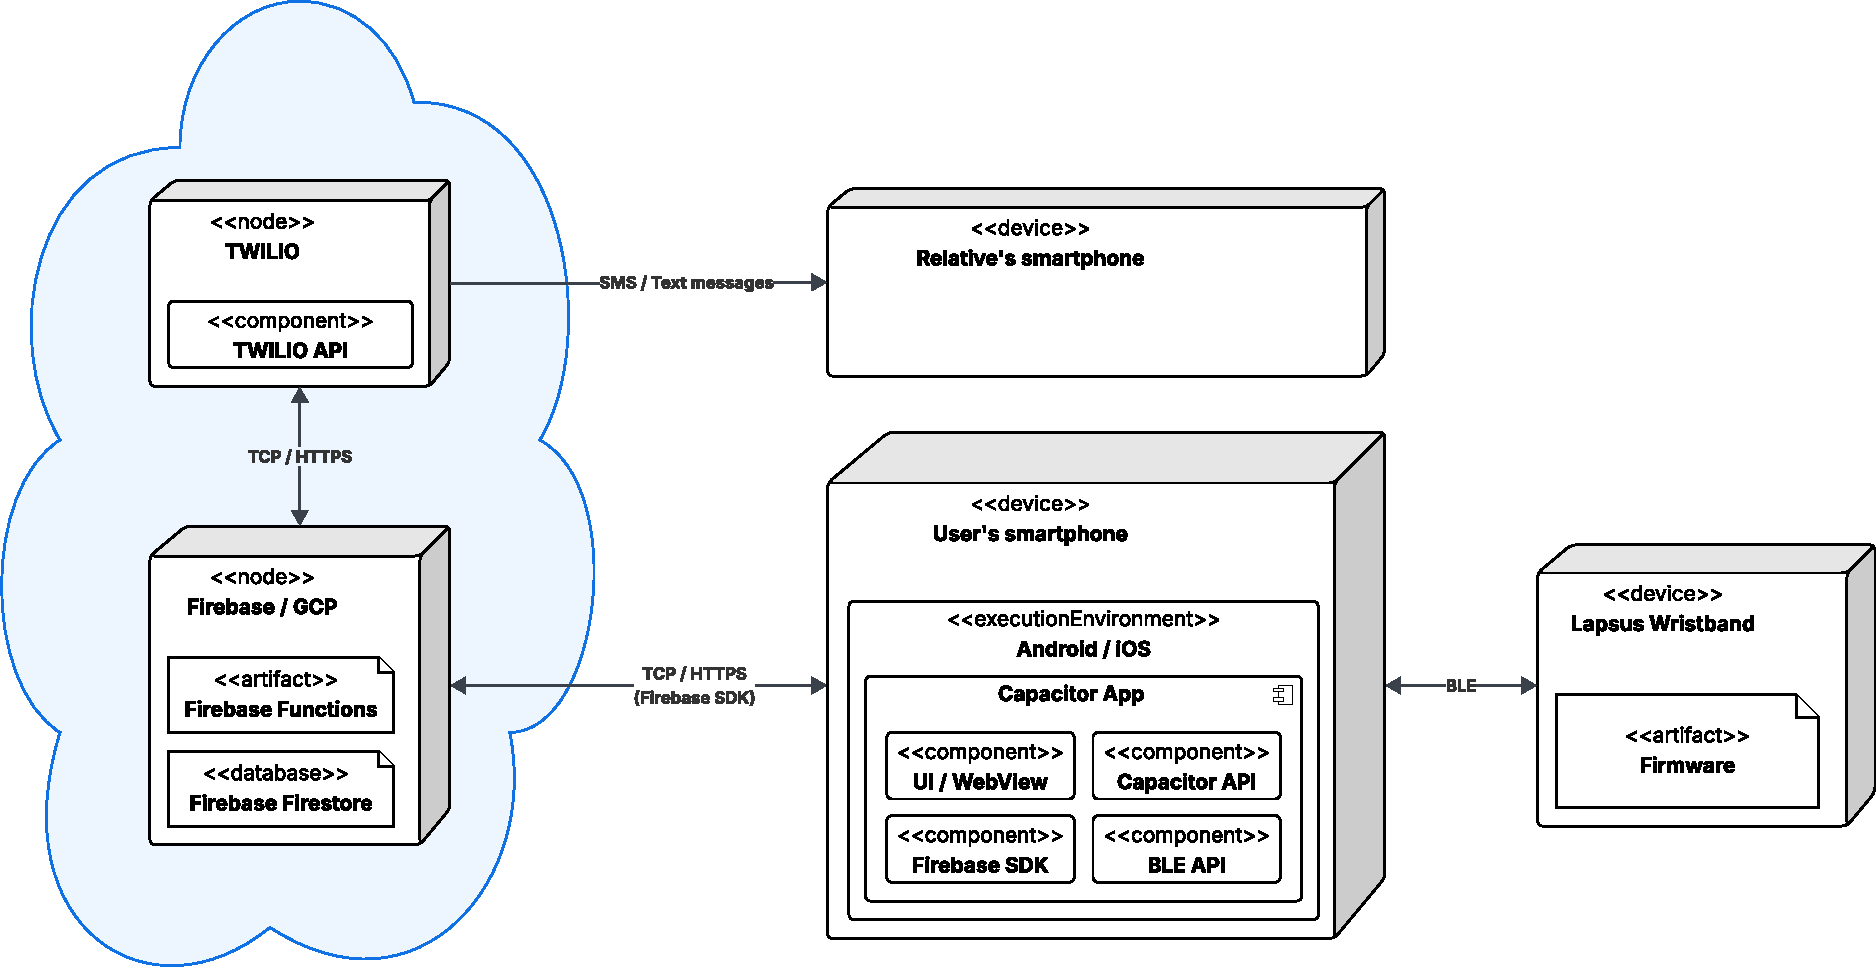
\includegraphics[width=1\linewidth]{Deployment-Diagram-Deployment-Diagram.pdf}
    \caption{Enter Caption}
    \label{fig:placeholder}
\end{figure}